% *** Authors should verify (and, if needed, correct) their LaTeX system  ***
% *** with the testflow diagnostic prior to trusting their LaTeX platform ***
% *** with production work. IEEE's font choices can trigger bugs that do  ***
% *** not appear when using other class files.                            ***
% The testflow support page is at:
% http://www.michaelshell.org/tex/testflow/


%%*************************************************************************
%% Legal Notice:
%% This code is offered as-is without any warranty either expressed or
%% implied; without even the implied warranty of MERCHANTABILITY or
%% FITNESS FOR A PARTICULAR PURPOSE!
%% User assumes all risk.
%% In no event shall IEEE or any contributor to this code be liable for
%% any damages or losses, including, but not limited to, incidental,
%% consequential, or any other damages, resulting from the use or misuse
%% of any information contained here.
%%
%% All comments are the opinions of their respective authors and are not
%% necessarily endorsed by the IEEE.
%%
%% This work is distributed under the LaTeX Project Public License (LPPL)
%% ( http://www.latex-project.org/ ) version 1.3, and may be freely used,
%% distributed and modified. A copy of the LPPL, version 1.3, is included
%% in the base LaTeX documentation of all distributions of LaTeX released
%% 2003/12/01 or later.
%% Retain all contribution notices and credits.
%% ** Modified files should be clearly indicated as such, including  **
%% ** renaming them and changing author support contact information. **
%%
%% File list of work: IEEEtran.cls, New_IEEEtran_how-to.pdf, bare_jrnl_new_sample4.tex,
%%*************************************************************************
\PassOptionsToPackage{unicode}{hyperref}
\PassOptionsToPackage{hyphens}{url}
\PassOptionsToPackage{dvipsnames,svgnames,x11names}{xcolor}
% Note that the a4paper option is mainly intended so that authors in
% countries using A4 can easily print to A4 and see how their papers will
% look in print - the typesetting of the document will not typically be
% affected with changes in paper size (but the bottom and side margins will).
% Use the testflow package mentioned above to verify correct handling of
% both paper sizes by the user's LaTeX system.
%
% Also note that the "draftcls" or "draftclsnofoot", not "draft", option
% should be used if it is desired that the figures are to be displayed in
% draft mode.
%
\documentclass[
  journal,
]{IEEEtran}%
% If IEEEtran.cls has not been installed into the LaTeX system files,
% manually specify the path to it like:
% \documentclass[journal]{../sty/IEEEtran}
\usepackage[cmex10]{amsmath}
\usepackage{amssymb}
\usepackage{iftex}
\ifPDFTeX
  \usepackage[T1]{fontenc}
  \usepackage[utf8]{inputenc}
  \usepackage{textcomp} % provide euro and other symbols
\else % if luatex or xetex
  \usepackage{unicode-math} % this also loads fontspec
  \defaultfontfeatures{Scale=MatchLowercase}
  \defaultfontfeatures[\rmfamily]{Ligatures=TeX,Scale=1}
\fi
%\usepackage{lmodern}
\ifPDFTeX\else
\fi
% Use upquote if available, for straight quotes in verbatim environments
\IfFileExists{upquote.sty}{\usepackage{upquote}}{}
\IfFileExists{microtype.sty}{% use microtype if available
  \usepackage[]{microtype}
  \UseMicrotypeSet[protrusion]{basicmath} % disable protrusion for tt fonts
}{}
\makeatletter
\parindent    1.0em
\ifCLASSOPTIONcompsoc
  \parindent    1.5em
\fi
\makeatother
\usepackage{xcolor}
\setlength{\emergencystretch}{3em} % prevent overfull lines

\setcounter{secnumdepth}{5}
% Make \paragraph and \subparagraph free-standing
\ifx\paragraph\undefined\else
  \let\oldparagraph\paragraph
  \renewcommand{\paragraph}[1]{\oldparagraph{#1}\mbox{}}
\fi
\ifx\subparagraph\undefined\else
  \let\oldsubparagraph\subparagraph
  \renewcommand{\subparagraph}[1]{\oldsubparagraph{#1}\mbox{}}
\fi


\providecommand{\tightlist}{%
  \setlength{\itemsep}{0pt}\setlength{\parskip}{0pt}}\usepackage{longtable,booktabs,array}
\usepackage{calc} % for calculating minipage widths
% Correct order of tables after \paragraph or \subparagraph
\usepackage{etoolbox}
\makeatletter
\patchcmd\longtable{\par}{\if@noskipsec\mbox{}\fi\par}{}{}
\makeatother
% Allow footnotes in longtable head/foot
\IfFileExists{footnotehyper.sty}{\usepackage{footnotehyper}}{\usepackage{footnote}}
\makesavenoteenv{longtable}
\usepackage{graphicx}
\makeatletter
\def\maxwidth{\ifdim\Gin@nat@width>\linewidth\linewidth\else\Gin@nat@width\fi}
\def\maxheight{\ifdim\Gin@nat@height>\textheight\textheight\else\Gin@nat@height\fi}
\makeatother
% Scale images if necessary, so that they will not overflow the page
% margins by default, and it is still possible to overwrite the defaults
% using explicit options in \includegraphics[width, height, ...]{}
\setkeys{Gin}{width=\maxwidth,height=\maxheight,keepaspectratio}
% Set default figure placement to htbp
\makeatletter
\def\fps@figure{htbp}
\makeatother

\usepackage{physics}
\usepackage[version=3]{mhchem}
\usepackage{orcidlink}
\usepackage{float}
\floatplacement{table}{htb}
\makeatletter
\@ifpackageloaded{caption}{}{\usepackage{caption}}
\AtBeginDocument{%
\ifdefined\contentsname
  \renewcommand*\contentsname{Table of contents}
\else
  \newcommand\contentsname{Table of contents}
\fi
\ifdefined\listfigurename
  \renewcommand*\listfigurename{List of Figures}
\else
  \newcommand\listfigurename{List of Figures}
\fi
\ifdefined\listtablename
  \renewcommand*\listtablename{List of Tables}
\else
  \newcommand\listtablename{List of Tables}
\fi
\ifdefined\figurename
  \renewcommand*\figurename{Fig.}
\else
  \newcommand\figurename{Fig.}
\fi
\ifdefined\tablename
  \renewcommand*\tablename{Table}
\else
  \newcommand\tablename{Table}
\fi
}
\@ifpackageloaded{float}{}{\usepackage{float}}
\floatstyle{ruled}
\@ifundefined{c@chapter}{\newfloat{codelisting}{h}{lop}}{\newfloat{codelisting}{h}{lop}[chapter]}
\floatname{codelisting}{Listing}
\newcommand*\listoflistings{\listof{codelisting}{List of Listings}}
\makeatother
\makeatletter
\makeatother
\makeatletter
\@ifpackageloaded{caption}{}{\usepackage{caption}}
\@ifpackageloaded{subcaption}{}{\usepackage{subcaption}}
\makeatother
\usepackage[skip=2pt,font=footnotesize]{caption}
%\captionsetup{format=myformat}
\ifLuaTeX
  \usepackage{selnolig}  % disable illegal ligatures
\fi
\IfFileExists{bookmark.sty}{\usepackage{bookmark}}{\usepackage{hyperref}}
\IfFileExists{xurl.sty}{\usepackage{xurl}}{} % add URL line breaks if available
\urlstyle{same} % disable monospaced font for URLs
\hypersetup{
  pdftitle={Optimizing Energy Market Trading with Conformal Predictions and Conditional Value at Risk},
  pdfauthor={Daniel Moore; Laila Saleh},
  pdfkeywords={Julia, Flux, LSTM, Conformal Prediction, conditional
value at risk, renewable energy, energy
markets, optimization, revenue, risk management},
  colorlinks=true,
  linkcolor={blue},
  filecolor={Maroon},
  citecolor={Blue},
  urlcolor={Blue},
  pdfcreator={LaTeX via pandoc}}

% *** Do not adjust lengths that control margins, column widths, etc. ***
% *** Do not use packages that alter fonts (such as pslatex).         ***
% There should be no need to do such things with IEEEtran.cls V1.6 and later.
% (Unless specifically asked to do so by the journal or conference you plan
% to submit to, of course. )


% correct bad hyphenation here
\hyphenation{op-tical net-works semi-conduc-tor}

%
% paper title
% can use linebreaks \\ within to get better formatting as desired
% Do not put math or special symbols in the title.
% paper title
% can use linebreaks \\ within to get better formatting as desired
% Do not put math or special symbols in the title.
\title{Optimizing Energy Market Trading with Conformal Predictions and
Conditional Value at Risk}

\author{
Daniel Moore
and~Laila Saleh%
\thanks{Daniel Moore is with Industrial and Systems Engineering, Rutgers
University%
}
%by-author.affiliations
\thanks{Laila Saleh is with Industrial and Systems Engineering, Rutgers
University%
}
%by-author.affiliations
}
\begin{document}

% The paper headers

% use for special paper notices

% make the title area
\maketitle

% As a general rule, do not put math, special symbols or citations
% in the abstract or keywords.
\begin{abstract}
We optimized the market trading of a renewable energy generation
operator with conditional value at risk based on probabilistic forecasts
made with a conformalized Long Short-term Memory (LSTM) recurrent neural
network. This work demonstrates an end-to-end workflow of how field data
can be ingested, analyzed, and exploited to reduce risk exposure for the
operator. This is financially beneficial to the individual operator, but
taken to a large scale this methodology increases the incentive for
renewable generation participation which should drive cost and emissions
down. This work used only eight features with favorable results, so it
is expected that further studies and more advanced models with the same
architecture would provide better yield.
\end{abstract}
% Note that keywords are not normally used for peerreview papers.
\begin{IEEEkeywords}
Julia, Flux, LSTM, Conformal Prediction, conditional value at
risk, renewable energy, energy markets, optimization, revenue, risk
management
\end{IEEEkeywords}

% For peer review papers, you can put extra information on the cover
% page as needed:
% \ifCLASSOPTIONpeerreview
% \begin{center} \bfseries EDICS Category: 3-BBND \end{center}
% \fi
%
% For peerreview papers, this IEEEtran command inserts a page break and
% creates the second title. It will be ignored for other modes.
% \IEEEpeerreviewmaketitle


\section{Introduction}\label{introduction}

The
\href{https://ieee-dataport.org/competitions/hybrid-energy-forecasting-and-trading-competition}{IEEE
Hybrid Energy Forecasting and Trading Competition} challenges
participants to make day-ahead, half-hourly probabilistic forecasts of
solar and wind energy production for a solar farm and Hornsea-1 Wind
Farm in the east of England with a combined 3.6 GW capacity and then
maximize revenue through commitment in the day-ahead market. Any
difference between the committed energy and actual energy is rewarded or
punished according to the single settlement price (SSP). The implied
task is to also forecast the market prices so that the operator can
reduce their risk exposure from both the energy production and market
prices.

\subsection{Motivation}\label{motivation}

This is an appropriate capstone project for this course as it applies
many topics covered ranging from unit commitment and energy market
trading to advanced predictive and prescriptive analytics for complex
and uncertain events. It is an interesting and practical opportunity to
wrestle with the available resources to make the best decisions for the
operator. Lastly, we find it a compelling problem because reducing the
risk for renewable energy generation operators will encourage more
participation and be of a net benefit to investors, consumers, and the
environment - a rare triple-win.

\subsection{Objectives}\label{objectives}

We will show an end-to-end workflow where we process data to train a
forecasting model and conformalize it so that its point forecasts can be
transformed into probabilistic forecasts. These forecasts enable us to
make market-trading decisions that consider the uncertainty in not only
energy production but also in the market itself. Finally, we will
demonstrate the financial benefit of leveraging the power of stochastic
optimization to reduce the risk exposure of the operator.

\subsection{Literature Review}\label{literature-review}

What have other people done

\section{Data Analysis}\label{data-analysis}

We have obtained datasets from two sources: the competition itself which
provides the energy production data through the
\href{https://www.rebase.energy/challenges/heftcom2024}{Rebase API} and
the \href{https://www.visualcrossing.com/weather-api}{VisualCrossing
API} which provides the weather data. The energy data details the solar
and wind energy production and the DAP and SSP in half-hourly
increments. The weather data is treated as historic for the period
preceding a given forecast and as a weather forecast for the forecast
horizon. If deployed, the model would need to operate only using
forecasted weather data. This approach is acceptable for this study as
24-hour-ahead weather forecasts are typically very accurate and we are
only incorporating basic weather features.

\subsection{Data Inisghts}\label{data-inisghts}

The tables below summarize the energy and weather data used throughout
this report. We have the amount of energy produced from solar, wind, and
combined total energy as well as the day-ahead and single settlement
prices. Combining the solar and wind energy results in a more
predictable value as we see the median total energy is greater than the
sum of the median solar and wind energy and the mean value is closer to
the median value. For the market prices we wee similar mean and median
values in the DAP and SSP but the domain of the SSP is much larger. Also
it is notable that both have negative values indicating there are times
of a surplus of energy which is penalized by the market.

\phantomsection\label{rebase-data-summary}
\begin{table}
\caption{Rebase Energy Data Summary}\tabularnewline

\centering
\begin{tabular}{r|ccccc}
    & variable & mean & min & median & max\\
    \hline
    & Symbol & Float32 & Float32 & Float64 & Float32\\
    \hline
    1 & Solar & 276.497 & 0.0 & 7.85413 & 1853.73 \\
    2 & Wind & 543.425 & 0.0 & 698.674 & 826.254 \\
    3 & TotalEnergy & 819.922 & 0.0 & 778.34 & 2367.19 \\
    4 & DAP & 56.0618 & -23.77 & 61.565 & 112.23 \\
    5 & SSP & 55.2193 & -88.0 & 55.595 & 177.71 \\
\end{tabular}
\end{table}

Examining the weather data, we see that verything but cloudcover is more
or less normally distributed. Cloudcover, however, is heavily skewed
towards being more cloudy as the mean is 71\% and the median is 92\%.
Being England, this lives up to expectations.

\phantomsection\label{weather-data-summary}
\begin{table}
\caption{Weather Data Summary}\tabularnewline

\centering
\begin{tabular}{r|ccccc}
    & variable & mean & min & median & max\\
    \hline
    & Symbol & Float32 & Float32 & Float64 & Float32\\
    \hline
    1 & temp & 8.54791 & -2.3 & 8.0 & 19.0 \\
    2 & windspeed & 16.9168 & 0.9 & 16.3 & 46.4 \\
    3 & winddir & 191.088 & 2.0 & 200.0 & 359.0 \\
    4 & cloudcover & 71.4654 & 0.0 & 91.6 & 100.0 \\
    5 & visibility & 14.4783 & 0.0 & 14.9 & 29.8 \\
\end{tabular}
\end{table}

\subsection{Data Visualizations}\label{data-visualizations}

In the following plots we examine first the day-ahead and then the
single settlement prices. The top plot shows the enitre history of the
data, the second provides a closer look at a single week. The bottom
plots show the prices vs.~temperature and total energy production with
the right side showing the daily seasonality. The relative variability
of the SSP compared to the DAP is highighted by the scales being the
same in the first and second plots.

For the DAP, we see a clear pattern with a few random dips in the price
but eventually returning to the mean. The week plot provides a clearer
look at the typical pattern. In the temperature plot we see that the
price tends to show the same general fluctuations regardless of the
price. There are two days around April 9th which seem to have low costs
associated with the warmest days. It is unclear whether this is a
coincidence. The bottom plot shows how the price changes with total
energy production. There is not a clear pattern in the monthly plot but
we do see that prices are at a constant high, but not peak, price when
energy production is the greatest. This is a direct consequence of solar
production and not a causation.

\begin{figure}

{\centering \includegraphics{EnergyProdConformalLSTM_files/mediabag/EnergyProdConformalLSTM_files/figure-pdf/monthly-dap-energy-price-plots-output-1.pdf}

}

\caption{Day Ahead Prices}

\end{figure}%

The SSP is a different story as the time-series is hardly
distinguishable from noise. We see the SSP fluctuates many times in a
given day and there is no evident seasonality. There is also no clear
pattern with temperature or total energy production. Finally, we note
that the SSP covers a much larger domain than the DAP and frequently
reaches near its extreme values.

\begin{figure}

{\centering \includegraphics{EnergyProdConformalLSTM_files/mediabag/EnergyProdConformalLSTM_files/figure-pdf/monthly-ssp-energy-price-plots-output-1.pdf}

}

\caption{Single Settlement Prices}

\end{figure}%

The violin plots with overlayed boxplots provide context for the trend
and seasonality for the market prices and energy production. First, we
can see there is no clear trend for any across the entire time frame.
Instead, we see cycles which hint at a dynamic relationship between the
prices and energy production. Note how in April we see a relatively
constant energy production associated with the most drastic decrease in
prices. The day of the week plots do hint at some trends, but nothing
strong enough to warrant a one-hot encoding. We do not have enough data
to determine whether it is a coincidence that Saturday has lower prices
or if there is actually some relationship that makes this a predictable
event. Finally, in the hourly plots we can finally observe a clear
trend. The DAP follows a close distribution at each hour of the day and
the change throughout the day is predicable. We can see a correlation
with the SSP, but still the SSP is more variable and not directly
correlated. Finally, we see that the total energy production follows a
clear pattern, but with upper and lower quantiles reaching the extreme
values indicating there are often enough times with very little or very
high production. Combining the wind and solar has resulted in a more
stable distribution.

\begin{figure}

{\centering \includegraphics{EnergyProdConformalLSTM_files/mediabag/EnergyProdConformalLSTM_files/figure-pdf/violin-plots-output-1.pdf}

}

\caption{Single Day, Weekly, and Daily Trends}

\end{figure}%

\section{Long Short-Term Memory
Model}\label{long-short-term-memory-model}

We used an LSTM Recurrent Neural Network (RNN) to predict the energy
production and market prices for the following day. RNNs are designed to
handle time-series data and LSTMs are a special type of RNN that can
learn long-term dependencies in the data. Combined with a dense neural
network, this model can remember (and forget) time-dependent
relationships and approximate the complex dynamics among the variables.

\subsection{Training}\label{training}

We used Julia's deep learning library, Flux, to build and train the
LSTM. We created a multi-target regressor to predict the energy
production and market prices in single timestep increments. All features
were normalized and time was encoded as a sine wave to capture the
cyclical nature of time.

\subsection{Performance}\label{performance}

Qualitatively, we observe the LSTM predictions are sensible and follow
the general characteristics of the target variables. It is able to
predict the Total Energy very well, but the market prices are not as
good.

\begin{figure}

{\centering 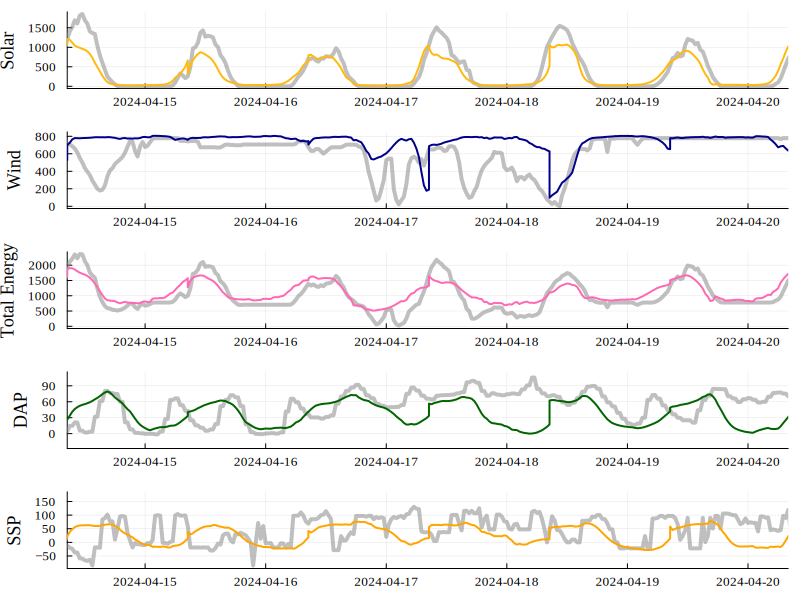
\includegraphics{EnergyProdConformalLSTM_files/mediabag/EnergyProdConformalLSTM_files/figure-pdf/plot-predictions-output-1.pdf}

}

\caption{Predictions}

\end{figure}%

We check the Mean Absolute and Root Mean Squared Error for all three
testing sets to ensure the model is not overfitting. The results are
shown the table below.

\phantomsection\label{test-error}
\begin{table}
\caption{Mean Absolute Error}\tabularnewline

\centering
\begin{tabular}{r|cccc}
    & feature & Train & Calib & Test\\
    \hline
    & Symbol & Float32 & Float32 & Float32\\
    \hline
    1 & Solar & 102.419 & 131.789 & 175.321 \\
    2 & Wind & 166.083 & 112.212 & 174.395 \\
    3 & TotalEnergy & 259.734 & 203.678 & 280.884 \\
    4 & DAP & 18.8602 & 20.8735 & 29.6261 \\
    5 & SSP & 34.4089 & 37.4783 & 46.8583 \\
\end{tabular}
\end{table}

\phantomsection\label{test-error-squared}
\begin{table}
\caption{Root Mean Square Error}\tabularnewline

\centering
\begin{tabular}{r|cccc}
    & feature & Train & Calib & Test\\
    \hline
    & Symbol & Float32 & Float32 & Float32\\
    \hline
    1 & Solar & 175.989 & 223.373 & 274.294 \\
    2 & Wind & 270.276 & 181.174 & 273.594 \\
    3 & TotalEnergy & 363.375 & 287.347 & 360.891 \\
    4 & DAP & 25.3194 & 27.2402 & 36.9338 \\
    5 & SSP & 42.9502 & 46.85 & 57.6788 \\
\end{tabular}
\end{table}

We see that the residuals are normally distributed with a mean of 0,
indicating we will be able to conformalize the model to obtain a
probabilistic forecast. Solar has most values at zero because the model
correctly predicts no solar energy production at night. We get around
this by using the combined energy as we don't explicitly have to know
the solar and the wind energy production.

\begin{figure}

{\centering 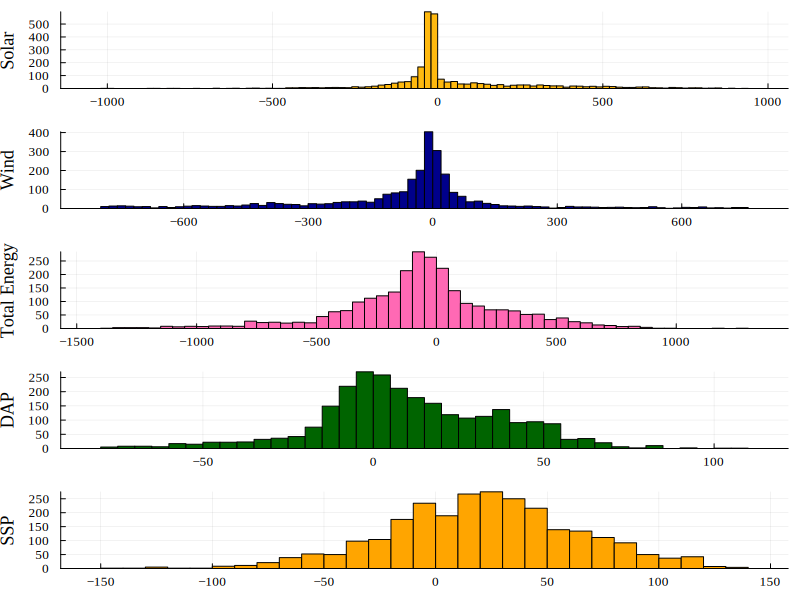
\includegraphics{EnergyProdConformalLSTM_files/mediabag/EnergyProdConformalLSTM_files/figure-pdf/plot-residuals-output-1.pdf}

}

\caption{Test Data Residuals}

\end{figure}%

\section{Conformalizing LSTM}\label{conformalizing-lstm}

The LSTM model has made predictions which capture the genaral behavior
of the target variables in terms of the time-dependent dynamics.
However, the model still has error that would make trading hazardous,
especially because we do not have a sense of how confident the model is
in its predictions.

\subsection{Implementation}\label{implementation}

Conformal predictions are an elegant solution to quantifying the
uncertainty of a point forecast model. It is emprically built from
calibration data which the model has not seen. For this regression task,
a simple residual nonconformity score is appropriate. We calculate the
absolute error for each prediction in the calibration data and save it
in a table for later reference. We can then retrieve the nonconformity
score for any prediction and \(\alpha\) level.

\subsection{Performance}\label{performance-1}

The nonconformity cumulative distribution functions are shown below. For
both the energy productiona and market prices, the nonconfomrity scores
grow exponentially once the quantile is past about 0.75. This indicates
that \(\alpha=0.75\) is a good choice for the confidence levels because
more than that and the range becomes too high while less than results in
too little coverage.

\begin{figure}

{\centering 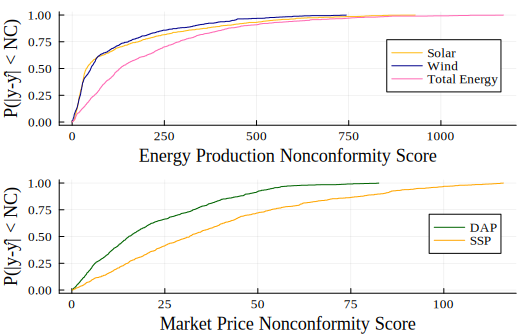
\includegraphics{EnergyProdConformalLSTM_files/mediabag/EnergyProdConformalLSTM_files/figure-pdf/plot-nonconformity-output-1.pdf}

}

\caption{Nonconformity Scores}

\end{figure}%

The coverage of the values for the calibration and test data at

\begin{figure}

{\centering 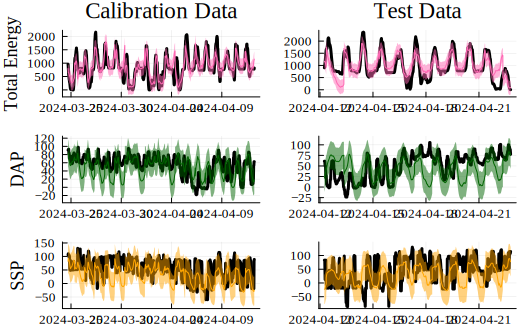
\includegraphics{EnergyProdConformalLSTM_files/mediabag/EnergyProdConformalLSTM_files/figure-pdf/coverage-output-1.pdf}

}

\caption{Prediction Coverage}

\end{figure}%

Finally, we confirm the coverage of the predictions for the test data at
\(\alpha=0.75\) for the total energy and market prices for the training,
calibration, and test data.

\phantomsection\label{coverage-table}
\begin{table}
\caption{Prediction Coverage}\tabularnewline

\centering
\begin{tabular}{r|cccc}
    & feature & Train & Calib & Test\\
    \hline
    & Symbol & Float64 & Float64 & Float64\\
    \hline
    1 & Solar & 0.820447 & 0.749448 & 0.685328 \\
    2 & Wind & 0.667526 & 0.749448 & 0.666023 \\
    3 & TotalEnergy & 0.643471 & 0.749448 & 0.611969 \\
    4 & DAP & 0.763746 & 0.749448 & 0.586873 \\
    5 & SSP & 0.766323 & 0.749448 & 0.656371 \\
\end{tabular}
\end{table}

We observe that the values are consistent for the training and
calibration data while the prediction intervals do not hold for the test
data where the coverage drops to as low as 0.62 for the DAP. Still, the
coverage for the Total Energy is at 0.72 which is acceptable. The
degradation of the coverage in the test data is likely due to increased
volatility in the markets which the model has not seen before.

\section{Market Trading}\label{market-trading}

With prediction for the energy production and market prices we can make
informed decisions about how much energy to commit to the day ahead
market. We will explore three strategies for comparison. It must be
assumed that the operator does not have the ability to store energy or
reduce energy production because we have not been provided that
information. If the operator could, they would opt to shut down
production if prices are expected to be negative. We cannot consider
this outcome because the data does not provide information on the cost
of shutting down production.

\begin{enumerate}
\def\labelenumi{\arabic{enumi}.}
\tightlist
\item
  Commit the point prediction of the total energy
\item
  Commit the confomral prediction of the total energy at a given
  \(\alpha\) level (as mentioned above we will use 0.75)
\item
  Commit the confomral prediction considering the joint probabilties of
  the total energy and market prices
\end{enumerate}

Revenue is calculated for this competition according to this formula
which approximates the impact of the difference between the energy
prediction and actual production on the settlement price.

\(Revenue = Trade*DAP + \Delta_E (SSP - 0.07 \Delta_E)\)
\(\Delta_E = Actual - Trade\)

\subsection{Revenue from Point
Prediction}\label{revenue-from-point-prediction}

The predicted total energy is used as the traded amount in the day ahead
market. Revenue is cacluated above using the actual total energy and the
actual market prices.

\subsection{Revenue from Conformal
Prediction}\label{revenue-from-conformal-prediction}

Here we determine the lower bound of the amount of energy to be produced
by subtracting the nonconformity score of the 75th quantile from the
point prediciton. We then trade the greater of this amount and zero as
negative values are not allowed. Revenue is caclualted as before.

\subsection{Revenue from Conditional Value at
Risk}\label{revenue-from-conditional-value-at-risk}

The shortcoming of the above methods are primarily that they do not
consider the market prices and the joint probability of the errors. We
must use joint probabilities to do so as the nonconformity scores of the
total energy, DAP, and SSP are correlated.

We have two options for capturing the joint probabilities. First, we
could assume these are multivariate normally distributed and we could
sample them as such. While convenient, it introduces additional
assumptions which may not be valid. Instead, we will sample the
residuals from the calibration data. For each timestep, we modify the
total energy and market predictions according to \(n\) samples from the
calibration data. For all values of the possible traded energy, we
evaluate the revenue for all sceanrios and find the amount to trade
which minimizes the expected shortfall. This process is depicted in the
plot below.

\begin{figure}

{\centering \includegraphics{EnergyProdConformalLSTM_files/mediabag/EnergyProdConformalLSTM_files/figure-pdf/cvar-plot-example-output-1.pdf}

}

\caption{Conditional Value at Risk}

\end{figure}%

The plot shows the revenue for each scenario as a scatter point colored
on the amount of energy expected to be produced. We have overlaid the
mean, median, 5th percentile value at risk, and the 5th percentile
conditional value at risk. Also as scatter points are the trade and
revenue amounts for a perfect energy production prediction, the point
forecast, and the conformal forecast. Finally, we see the large green
diamond indicating the revenue actually recieved for this time step at
the trade amount set by the conditional value at risk. We note how the
aggregation for the mean and value at risk smooths the curves to they
have a convex shape.

\subsection{Performance}\label{performance-2}

Below we examine the revenues for each trading strategy. THe top plot
shows that all strategies are typically making the ssame revnue but
there is one moment where the predictions all suffer a catastrophic
loss. The middle plot shows the cumulative revenue and we see over time
they all recover but the dip is pronounced. Lastly at the bottom there
is a plot which shows the relative cumulative value of each strategy
compared to the perfect prediction. Eventually, they all recover and
their values approach around 0.6 in the long run. Surprisingly the point
forecast is the best followed by the CVaR and finally the conformal
prediction.

\begin{figure}

{\centering 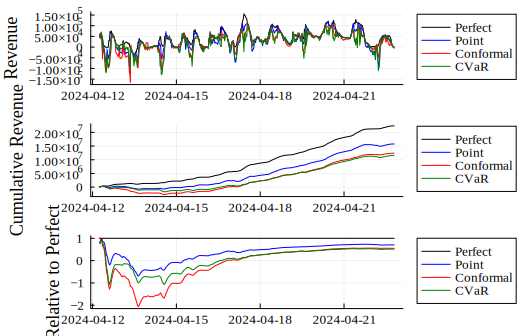
\includegraphics{EnergyProdConformalLSTM_files/mediabag/EnergyProdConformalLSTM_files/figure-pdf/revenue-plots-output-1.pdf}

}

\caption{Revnue vs.~Time}

\end{figure}%

\section{Conclusions}\label{conclusions}

Suggestions for future work 1. Include more data, especially demand
predictions 2. Include the cost of shutting down production 3. Predict a
trade amount which will maximize the revenue with some \(\alpha\) level
directly


% Can use something like this to put references on a page
% by themselves when using endfloat and the captionsoff option.
\ifCLASSOPTIONcaptionsoff
  \newpage
\fi

% trigger a \newpage just before the given reference
% number - used to balance the columns on the last page
% adjust value as needed - may need to be readjusted if
% the document is modified later
%\IEEEtriggeratref{8}
% The "triggered" command can be changed if desired:
%\IEEEtriggercmd{\enlargethispage{-5in}}

% Uncomment when use biblatex with style=ieee
%\renewcommand{\bibfont}{\footnotesize} % for IEEE bibfont size

\pagebreak[3]
% that's all folks
\end{document}

